\documentclass[thesis.tex]{subfiles}

\begin{document}
    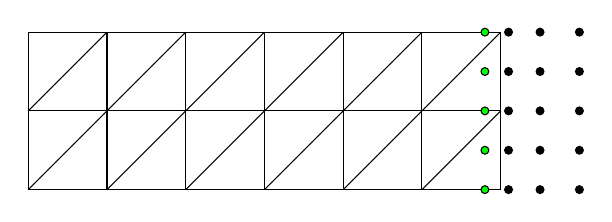
\begin{tikzpicture}[domain=-3:3]
        % сетка
        \draw (-5,-1) -- (-5,1) -- (1,1) -- (1,-1) -- cycle;
        \draw (-5,0) -- (1,0);
        \draw(-4,1) -- (-4,-1);
        \draw(-3,1) -- (-3,-1);
        \draw(-2,1) -- (-2,-1);
        \draw(-1,1) -- (-1,-1);
        \draw(0,1) -- (0,-1);
        \draw(-4,1) -- (-5,0);
        \draw(-3,1) -- (-5,-1);
        \draw(-2,1) -- (-4,-1);
        \draw(-1,1) -- (-3,-1);
        \draw(0,1) -- (-2,-1);
        \draw(1,1) -- (-1,-1);
        \draw(1,0) -- (0,-1);

        \node[draw,circle,inner sep=1pt,fill] at (2 ,1) {};
        \node[draw,circle,inner sep=1pt,fill] at (1.5 ,1) {};
        \node[draw,circle,inner sep=1pt,fill] at (2 ,0.5) {};
        \node[draw,circle,inner sep=1pt,fill] at (1.5 ,0.5) {};
        \node[draw,circle,inner sep=1pt,fill] at (2 ,0) {};
        \node[draw,circle,inner sep=1pt,fill] at (1.5 ,0) {};
        \node[draw,circle,inner sep=1pt,fill] at (2 ,-1) {};
        \node[draw,circle,inner sep=1pt,fill] at (1.5 ,-1) {};
        \node[draw,circle,inner sep=1pt,fill] at (2 ,-0.5) {};
        \node[draw,circle,inner sep=1pt,fill] at (1.5 ,-0.5) {};
        \node[draw,circle,inner sep=1pt,fill] at (1.1 ,1) {};
        \node[draw,circle,inner sep=1pt,fill] at (1.1 ,0.5) {};
        \node[draw,circle,inner sep=1pt,fill] at (1.1 ,0) {};
        \node[draw,circle,inner sep=1pt,fill] at (1.1 ,-1) {};
        \node[draw,circle,inner sep=1pt,fill] at (1.1 ,-0.5) {};
        \node[draw,circle,inner sep=1pt,fill=green] at (0.8 ,1) {};
        \node[draw,circle,inner sep=1pt,fill=green] at (0.8 ,0.5) {};
        \node[draw,circle,inner sep=1pt,fill=green] at (0.8 ,0) {};
        \node[draw,circle,inner sep=1pt,fill=green] at (0.8 ,-1) {};
        \node[draw,circle,inner sep=1pt,fill=green] at (0.8 ,-0.5) {};
    \end{tikzpicture}
\end{document}
